
\documentclass[aps,floatfix,prd,showpacs]{revtex4}
%\documentclass[aps,floatfix,prd,showpacs,twocolumn]{revtex4}
\usepackage{graphicx}% Include figure files
\usepackage{dcolumn}% Align table columns on decimal point
\usepackage{bm}% bold math

\voffset 1.0cm

\begin{document}


\title{Comparison of Computer Simulation Methods for Predicting Chemical Reactions}
\author{Graham Gibson}
\affiliation{
IBM,
Austin TX,
78723,
USA.}

\date{\today}

\begin{abstract}

In this paper we compare two primary methods of predicting basic organic chemistry reaction predictions. We analyze two types of models, an NLP based Neural Network and an agent based model. We compare and contrast the complexity, accuracy, and generalizability of both models as applied to predicting organic chemistry reactions. Two basic reaction mechanisms are explored, Elimination and Addition reactions.  These two mechanisms are simple but fundamental to the set of organic reactions, as many more complicated reactions use this mechanisms as intermediates.  We first verify the model on an alkene halogen addition reaction and then investigate the models generalizability to the elimination reaction. 


\end{abstract}
\pacs{PACS numbers go here. These are classification codes for your  research. See {\tt http://publish.aps.org/PACS/} for more info.}
\maketitle

\section{Introduction}

The problem of reliably predicting organic chemical reactions is vital in computation chemistry and biology. A model that is able to describe 3-dimension conformations of reactions would go a long way towards solving the more complicated protein folding problem. Finding such a solution would have extremely beneficial consequences in the area of targeted drug development and computational medicine. Such a solution would also drastically reduce drug development time and help eliminate clinical trail risk.

Traditional computational chemistry approaches have involved analyzing the potential energy surface of the atoms in the n-molecule system. The energy surface contains an array of parameters from 3-d cartesian coordinates, to electronegativity, to electron-electron repulsion. Finding the most likely product is equivalent to finding minima in the energy surface using tradition techniques like gradient descent. This method is often termed molecular dynamics . 
A second approach that is frequently taken is to go deeper into the reaction and look at the driving quantum mechanical principles that are at play. These methods use a combination of approximation techniques to guess the Hamiltonian of an atom and analytically solve for the orbital energy. This allows one to identify reactive orbitals very precisely. The two primary methods are called Hartree-Fock and Density Functional Theory. 
Although these approaches are invaluable in their description of the energy of chemical reactions, they are both quite complicated and computationally involved. The quantum mechanical approaches are extremely resource intensive as the involve the approximation of complicated integrals and matrix multiplications. It also appears that both methods are essentially overkill when trying predict the result of organic reactions. The reasoning behind this is that chemistry students begin studying reaction mechanisms and gain the ability to predict basic reactions long before they learn about solving Hamiltonian equations. Organic chemistry textbooks focus on what we call the "grammar" of organic chemistry. This involves  studying common reaction mechanisms and patterns of behavior of common functional groups such as OH, COOH, alkenes etc. Organic chemistry students learn chemistry as a combination of a language of interacting words and they verify reaction products as syntactically and semantically valid under such language. Using this view we can define two separate higher level approaches to predicting chemical reactions.

\subsubsection{First Approach: Language Based Modeling }
Continuing with the idea of modeling organic reactions as language over the alphabet of atoms, predicting a chemical reaction has a natural analogy between verifying if a sentence is valid in a given language. This problem has been studied in depth in the field of computer science and has been most successfully modeled by using recursive neural networks (RNNs) such as the Long Short Term Memory network architecture. This architecture maintains state of the neural network by copying the hidden state $H_{t-1}$ to the hidden state $H_{t}$ using a series of memory gates. LSTM networks have gained a lot of popularity in the computer science community for their ability to remember context from many time steps previous to the current because of this copying of hidden layer state. A common LSTM network approach to the problem of machine translation is depicted below as in \cite(-sequence-to-sequence-learning-with-neural-networks) 

\section{Results}
Including figures, tables, and equations is easy. Latex also permits easy reference to document elements (figures, tables, sections) with the \begin{verbatim}\ref\end{verbatim} command\ref{fig1}. Citations are made with the \begin{verbatim}\cite\end{verbatim} command\cite{lamport}. 

\begin{figure}[ht]
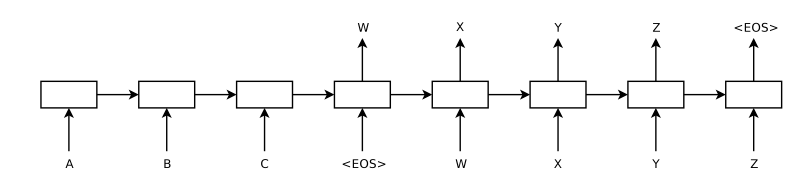
\includegraphics[width=7cm,angle=-90]{fig1.png}
\caption{You will need to include the package graphicx to be able to make figures like this.}
\label{fig1}
\end{figure}

\begin{figure}[ht]
%\includegraphics[width=7cm,angle=-90]{linear_q_eq_0.ps}
\caption{You will need to include the package graphicx to be able to make figures like this.}
\label{fig1}
\end{figure}

A simple table.

\begin{table}[ht]
\caption{$X(3872)$ Discovery Modes.}
\label{XmodesTab}
\begin{tabular}{cclccl}
\hline
mass & width & production/decay mode & events & significance & experiment\\
\hline
\hline
$3872.0 \pm 0.6 \pm 0.5$  & $< 2.3$ 90\% C.L.  & $B^\pm \to K^\pm X \to K^\pm \pi^+ \pi^- J/\psi$   &  $25.6 \pm 6.8$ & $10 \sigma$     & Belle\\
$3871.3 \pm 0.7 \pm 0.4$  & resolution & $p\bar p \to  X \to \pi^+ \pi^- J/\psi$   &  $730 \pm 90$ & $11.6 \sigma$  & CDFII\\
$M(J/\psi) + 774.9 \pm 3.1 \pm 3.0$ & resolution & $p\bar p \to X \to \pi^+\pi^-J/\psi$ & $522 \pm 100$ & $5.2 \sigma$  & D{\O} \\
$3873.4 \pm 1.4$  &  --  & $B^- \to K^- X \to K^- \pi^+ \pi^- J/\psi$   &  $25.4 \pm 8.7$ &$3.5 \sigma$ & BaBar\\
\hline
\hline
\end{tabular}
\end{table}

And a sample equation (Eq. \ref{XCD}).

\begin{equation}
\Gamma(X \to \alpha\beta D) = \int {d^3Q\over (2\pi)^3}  \Gamma(C\to \alpha\beta) {|\tilde T(Q)|^2 \over
(M(X) - E_{CD}(Q))^2 + \Gamma_C^2/4}
\label{XCD}
\end{equation}





\section{Conclusions}

Man, latex is great!

\acknowledgments
The author is grateful to Donald Knuth for inventing tex, and making publication quality typesetting a reality for scientists around the world.


\begin{thebibliography}{99}

\bibitem{lamport}
 {\sl LaTeX : A Documentation Preparation System User's Guide and Reference Manual}, Leslie Lamport [1994] (ISBN: 0-201-52983-1) pages: xvi+272.

\bibitem{latt}
I.M. Smart {\it et al.}, J. Plumb Phys. {\bf 50}, 393 (1983).

\end{thebibliography}

\end{document}



